\begin{titlepage}
	\parindent0pt
	
	\begin{tikzpicture}[remember picture, overlay, shift={(current page.south west)}]
		\fill [BurntOrange!5] (current page.north west) rectangle (current page.south east); 
		\fill [BurntOrange] (current page.north west) rectangle (21,28.7); 
		\fill [OliveGreen!80] (current page.north west) -- (0,0) -- (1,0) -- (1,28.7) -- cycle; 
	\end{tikzpicture}
	
	\begin{center}
		{\huge\scshape Travaux personnels encadrés}
		
		\addvspace{.5cm}
		
		du
		
		\addvspace{.5cm}
		
		{\Large\scshape Lycée François Rabelais de Chinon}
		
		{\large Baccalauréat scientifique, option sciences de l'ingénieur}
		
		\vfill
		
		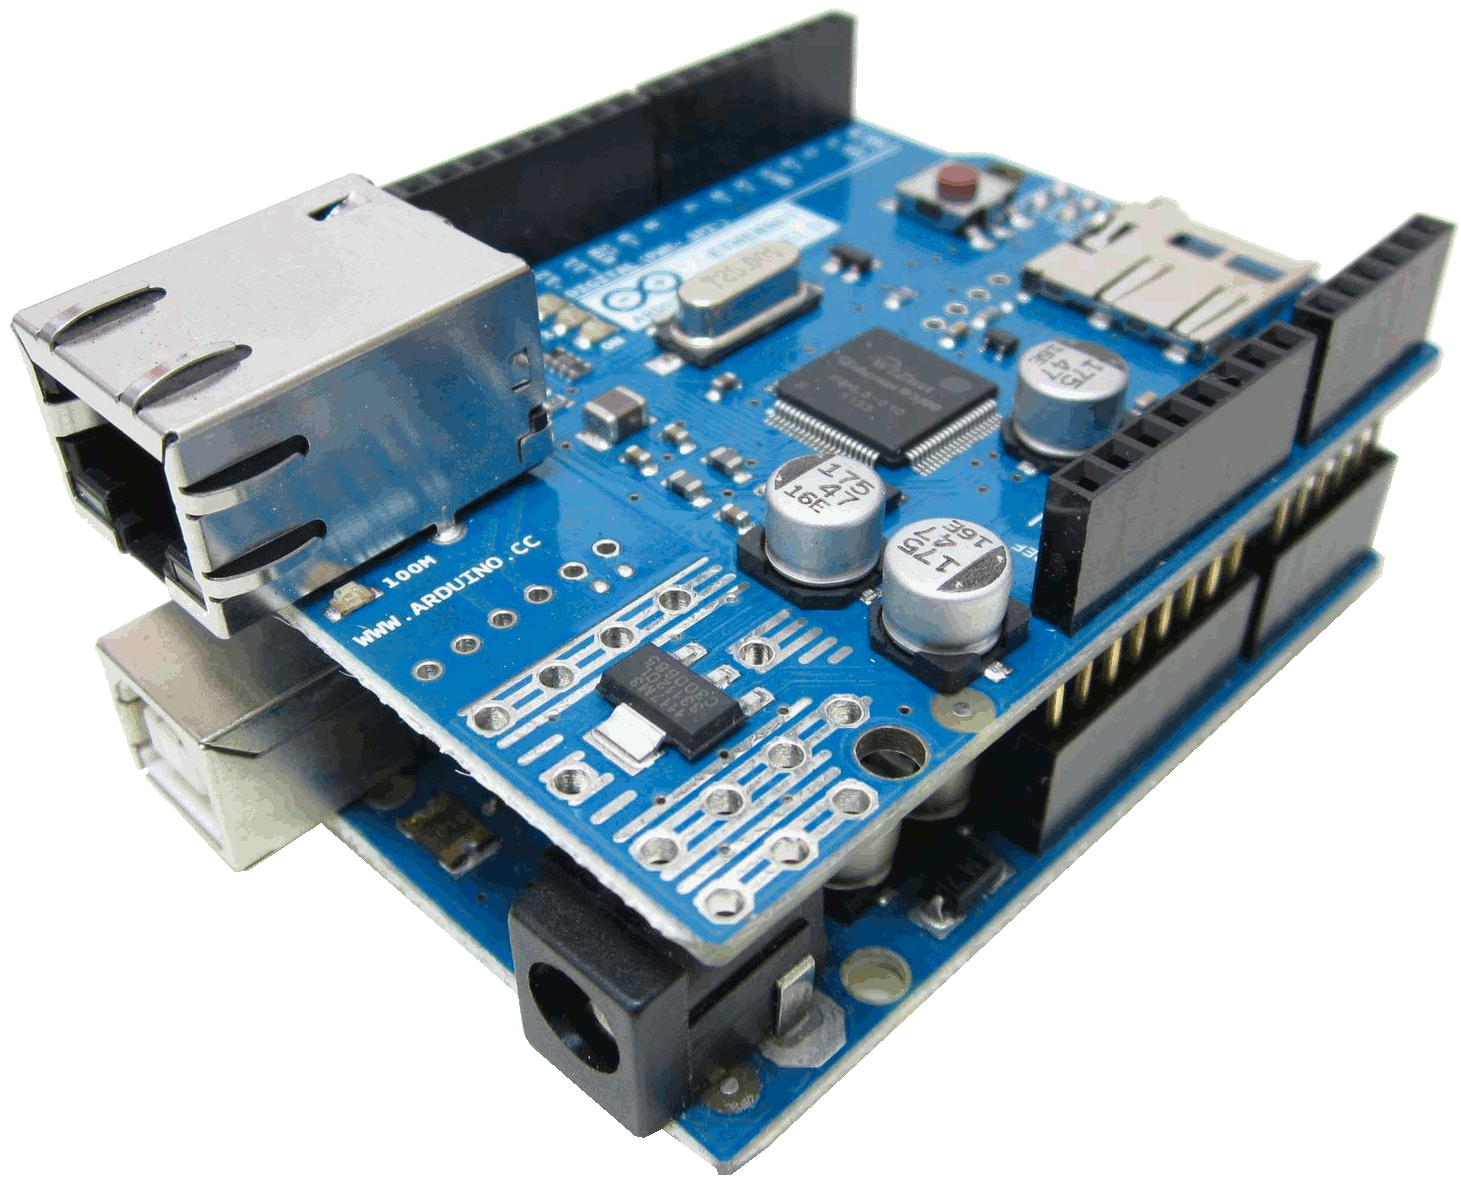
\includegraphics[width=.5\linewidth]{Images/Arduino_Ethernet_Shield}
		
		\vfill
		
		{\Large Thème du TPE : \og Avancée scientifique et réalisations techniques \fg}
		
		\vfill
		
		\hrule height .5mm
		
		\addvspace{.5cm}
		
		{\huge\bfseries Comment relever des données météorologiques et les transmettre sur un espace accessible par tous ?}
		
		\addvspace{.5cm}
		
		\hrule height .5mm
		
		\vfill
		
		
\includegraphics[width=.5\linewidth]{Images/Logo_Arduino}
		
		\vfill
	\end{center}
	
	Soutenu le 25 mars 2015
	
	\vfill
	
	{\large
	\begin{minipage}{.6\linewidth}
		Encadré par
		
		M. \bsc{Labourdette} : professeur de sciences de l'ingénieur
		
		M. \bsc{Guibert} : professeur de sciences de l'ingénieur
	\end{minipage}%
	\begin{minipage}{.4\linewidth}
		\flushright
		Présenté par
		
		Téofil \bsc{Adamski}
		
		Remi \bsc{Bruyère}
		
		Sammy \bsc{Plat}
		
		Clément \bsc{Bidault}
	\end{minipage}}
\end{titlepage}